\documentclass[11pt,a4paper,english]{article}
  \usepackage[latin1]{inputenc}
  \usepackage{amsmath,amsfonts,amssymb}
  \usepackage{enumitem}
  \usepackage{fullpage}
  \usepackage{graphicx}
  \usepackage{tabto}
  \usepackage{etoolbox}
  \usepackage{hyperref}
  \usepackage{minted}
  \usepackage{parskip}
  \usepackage[font=small,labelfont=bf]{caption}
  \newcommand\numberthis{\addtocounter{equation}{1}\tag{\theequation}}
  \renewcommand{\labelenumii}{\theenumii}
  \renewcommand{\theenumii}{\theenumi.\arabic{enumii}.}

  \title{Algorithmic Methods of Data Mining - Assignment 2}
  \author{Maksad Donayorov}

  \begin{document}
    \maketitle
    \definecolor{bg}{rgb}{0.95,0.95,0.95}

    \begin{enumerate}
      \item \textbf{Problem:} \textit{Bag of words:}
        \begin{enumerate}
          \item \textbf{Question:} \textit{Jaccard coefficient to bags is meaningful and well-motivated:}\\
            Jaccard coefficient is used for comparing the similarity and diversity of sets. As we are using a finite set to represent "bag of words" the extention of Jaccard index to bag is meaningful and well-motivated.

            For example: assume that we have two documents which are not similar and represented by sets: $A = \{(x, 2), (y, 3)\}$ and $B = \{(x, 1),(z, 3)\}$. The Jaccard coefficient for these documents will be:
            \begin{align*}
              J(A, B) = \frac{\|A \cap B\|}{\|A \cup B\|} =
              \frac{ \| \{x,x,y,y,y\} \cap \{x,z,z,z\} \| }{ \| \{x,x,y,y,y\} \cup \{x,z,z,z\} \| } & = \\
              \frac{ \| \{x\} \| }{ \| \{ x,x,y,y,y,z,z,z \} \| } & = \frac{1}{8} = 0.125
            \end{align*}
            As we can see the Jaccard index does prove that these two documents are not similar.
            On the contrary, if we take two exactly the same bags: $A = \{(x, 2), (y, 1)\}$ and $B = \{(x, 2),(y, 1)\}$. The the Jaccard index will be:
            \begin{align*}
              J(A, B) = \frac{\|A \cap B\|}{\|A \cup B\|} =
              \frac{ \| \{x,x,y\} \cap \{x,x,y\} \| }{ \| \{x,x,y\} \cup \{x,x,y\} \| } & = \\
              \frac{ \| \{x,x,y\} \| }{ \| \{ x,x,y \} \| } & = \frac{1}{1} = 1
            \end{align*}
            And again we can prove by Jaccard index that these two documents are exactly the same. Consequently, we can say that the extension of the Jaccard coefficient to bags, is
            meaningful and well-motivated.

          \item \textbf{Question:} \textit{Design a family of hash functions $\mathcal{F}$:}\\
            As mentioned in the part $1.1$ the Jaccard index measures how similar two sets are. Therefore, we can use \textbf{min-hash} locality-sensitive hashing scheme for Jaccard coefficient to bags.

            Now coming back to the prove that min-hash function does satisfies this $Pr[f(A)= f(B)]=J(A,B)$ equality. As always, it is the best to have a good intuition and for that we can look at an example. Let's assume we have two bags:
            \begin{align*}
              A = \{ (x,2), (y,2), (z,1) \} \\
              B = \{ (x,2), (z,1) \} \\
            \end{align*}
            Let's now take the union of $A$ and $B$.
            \begin{align*}
              C = A \cup B = \{ (x,2), (y,2), (z,1) \} = \{ x_0, x_1, y_2, y_3, z_4 \} \\
            \end{align*}
            This union shows us that all the elements that $A$ and $B$ have and we can use this set in our "hash table". But before that let's think of some hash function. Based on the book a good hash function is the one that has a modulo of a prime number that is bigger than the number of elements in the union set $C$. Since we have 5 elements in $C$ we can choose $7$ for our modulo and create some hash functions:
            \begin{align*}
               (i + 1) & \ mod \ 7 \\
              2(i + 1) & \ mod \ 7 \\
              (i + 13) & \ mod \ 7
            \end{align*}
            Following these hash functions we can generate a hash table and populate it with the value of hash functions where $i$ is the value of index: \\
            \begin{center}
              \begin{tabular}{c | c | c || c | c | c}
                $i$   & $A$ & $B$ & $(i + 1) \ mod \ 7$ & $2(i + 1) \ mod \ 7$ & $(i + 13) \ mod \ 7$ \\ \hline \hline
                $x_0$ &  1  &  1  &       1       &       2        &      5         \\
                $x_1$ &  1  &  1  &       2       &       3        &      0         \\
                $y_2$ &  1  &  0  &       3       &       6        &      1         \\
                $y_3$ &  1  &  0  &       4       &       1        &      2         \\
                $z_4$ &  1  &  1  &       5       &       3        &      3         \\  \hline
                      &     &     &     $h_1$     &     $h_2$      &     $h_3$      \\
              \end{tabular}
            \end{center}

            The next step would be creating a signature matrix based the hash table:
            \begin{center}
              \begin{tabular}{|c | c c |}\hline
                $i=0$ & $A$ & $B$ \\ \hline
                $h_1$ &  1  &  1  \\
                $h_2$ &  2  &  2  \\
                $h_3$ &  5  &  5  \\  \hline
              \end{tabular}
              \begin{tabular}{|c | c c |}\hline
                $i=1$ & $A$ & $B$ \\ \hline
                $h_1$ &  1  &  1  \\
                $h_2$ &  2  &  2  \\
                $h_3$ &  0  &  0  \\  \hline
              \end{tabular}
              \begin{tabular}{|c | c c |}\hline
                $i=2$ & $A$ & $B$ \\ \hline
                $h_1$ &  1  &  1  \\
                $h_2$ &  2  &  2  \\
                $h_3$ &  0  &  0  \\  \hline
              \end{tabular}
              \begin{tabular}{|c | c c |}\hline
                $i=3$ & $A$ & $B$ \\ \hline
                $h_1$ &  1  &  1  \\
                $h_2$ &  1  &  2  \\
                $h_3$ &  0  &  0  \\  \hline
              \end{tabular}
              \begin{tabular}{|c | c c |}\hline
                $i=4$ & $A$ & $B$ \\ \hline
                $h_1$ &  1  &  1  \\
                $h_2$ &  1  &  2  \\
                $h_3$ &  0  &  0  \\  \hline
              \end{tabular}
            \end{center}
            We are interested in the signature matrix when $i=4$, as that's the last index and it will give us the similarity of $A$ and $B$.
            \begin{align*}
              \begin{tabular}{|c | c c | c | }\hline
                $i=4$ & $A$ & $B$ & similarity\\ \hline
                $h_1$ &  1  &  1  & 1\\
                $h_2$ &  1  &  2  & 0\\
                $h_3$ &  0  &  0  & 1\\  \hline
              \end{tabular}
            \end{align*}
            The $similarity$ column shows us that 2 out 3 hash function found $A$ to be similar to $B$. Which is:
            \begin{align*}
              minHash(A,B) = \dfrac{2}{3} = 0.666\bar{6}
            \end{align*}
            To compare the correctness of our calculations we can have a look at Jaccard coefficient for $A$ and $B$.
            \begin{align*}
              J(A,B) = \dfrac{\| A \cap B \|}{\| A \cup B \|} =
              \frac{ \| \{ x,x,z\} \| }{ \| \{ x,x,y,y,z \} \| } = \frac{3}{5} = 0.6
            \end{align*}

            As you can see $J(A,B) \approx minHash(A,B) \approx 0.6$. By defining more hash functions we can decrease this approximation. Consequently, we proved that the equality holds.

          \item \textbf{Question:} \textit{Provide pseudo-code $\mathcal{F}$:}\\
            The algorithm is pretty straight forward:
            \begin{enumerate}
              \item for sets $A$, $B$ and etc that represent documents
              \item calculated set $C$, such that $C = A \cup B \cup ...$
              \item shuffle set $C$
              \item sample from C the minimum element in permutation
              \item populate signature matrix
              \item compute similarity of documents by the last signature matrix's values
            \end{enumerate}

            \begin{minted}[bgcolor=bg,linenos,fontsize=\small,autogobble]{js}
              sample = generate a sample from Union set
              Row = good items of sample

              for row in Row:
                for hash_func in hash_functions:
                  compute hash_func(row)
                  for column in S:
                    if hash_func(row) < signature(S,i):
                      sig_matrix(i) = hash_func(row)

              // query
              quer = new_doc
              for row in length(quer):
                for hash in hash_functions:
                  hash = compute hash_func(row)
                  if hash < signature(S,i):
                    sig_matrix(i) = hash

              similarity = compare(new_doc, sig_matrix)
            \end{minted}
        \end{enumerate}

      \item \textbf{Problem:} $\mathcal{O}(\log{w}\ \log{n})$: \\
        Before analyzing the complexity and responding to the question it could be nice to see an algorithm that finds the $max$ number in an array. Such algorithm can be easily written in python, that gives us a clear picture of how the computation is done:
        \begin{minted}[bgcolor=bg,linenos,fontsize=\small,autogobble]{js}
          def get_max(arr):
            max_num = -1
            for el in arr:
              if max_num < el:
                max_num = el
            return max_num
        \end{minted}

        The best case for finding the $max$ element is when the first element is bigger than all of the other elements of $X$, which has complexity of $\mathcal{O}(1)$. And the worst case is when the last element is the largest and all the consecutive numbers proceed from small to large. This case has a complexity of $\mathcal{O}(n)$. The tricky part is the average case, where we have to compute the complexity for \textit{the number of times that max is assigned to an element}.

        Assuming that $X[1,2,3...m]$ is drawn independently and uniformly at random from the interval $(0,1)$, the expected value will be:
        \begin{align*}
          E[x] = \sum\limits_{i=1}^{m} Pr(X_i)
        \end{align*}
        Where $Pr(X_i)$ is the probability of the \textit{i-th} element being the $max$ element in $X[1,2,3...m]$. To have a better intuition of what could be the probability of \textit{i-th} element we can have a look at different size of $m$:
        \begin{align*}
          Pr(x_1) & = 1 \\
          Pr(x_2) & = \frac{1}{2} \\
          Pr(x_3) & = \frac{1}{3} \\
                  & ... \\
          Pr(x_m) & = \frac{1}{m} \\
        \end{align*}
        Looking at this we can infer that the expected value can be calculated as:
        \begin{align*}
          E[x] = 1 + \frac{1}{2} + \frac{1}{3} + ... + \frac{1}{m} = \sum\limits_{i=1}^{m}{\frac{1}{i}} \approx \log{m}
        \end{align*}
        Consequently, we can conclude that $max = X[i]$ will be executed $\mathcal{O}(\log m)$ times, on expectation.

        \begin{center}
          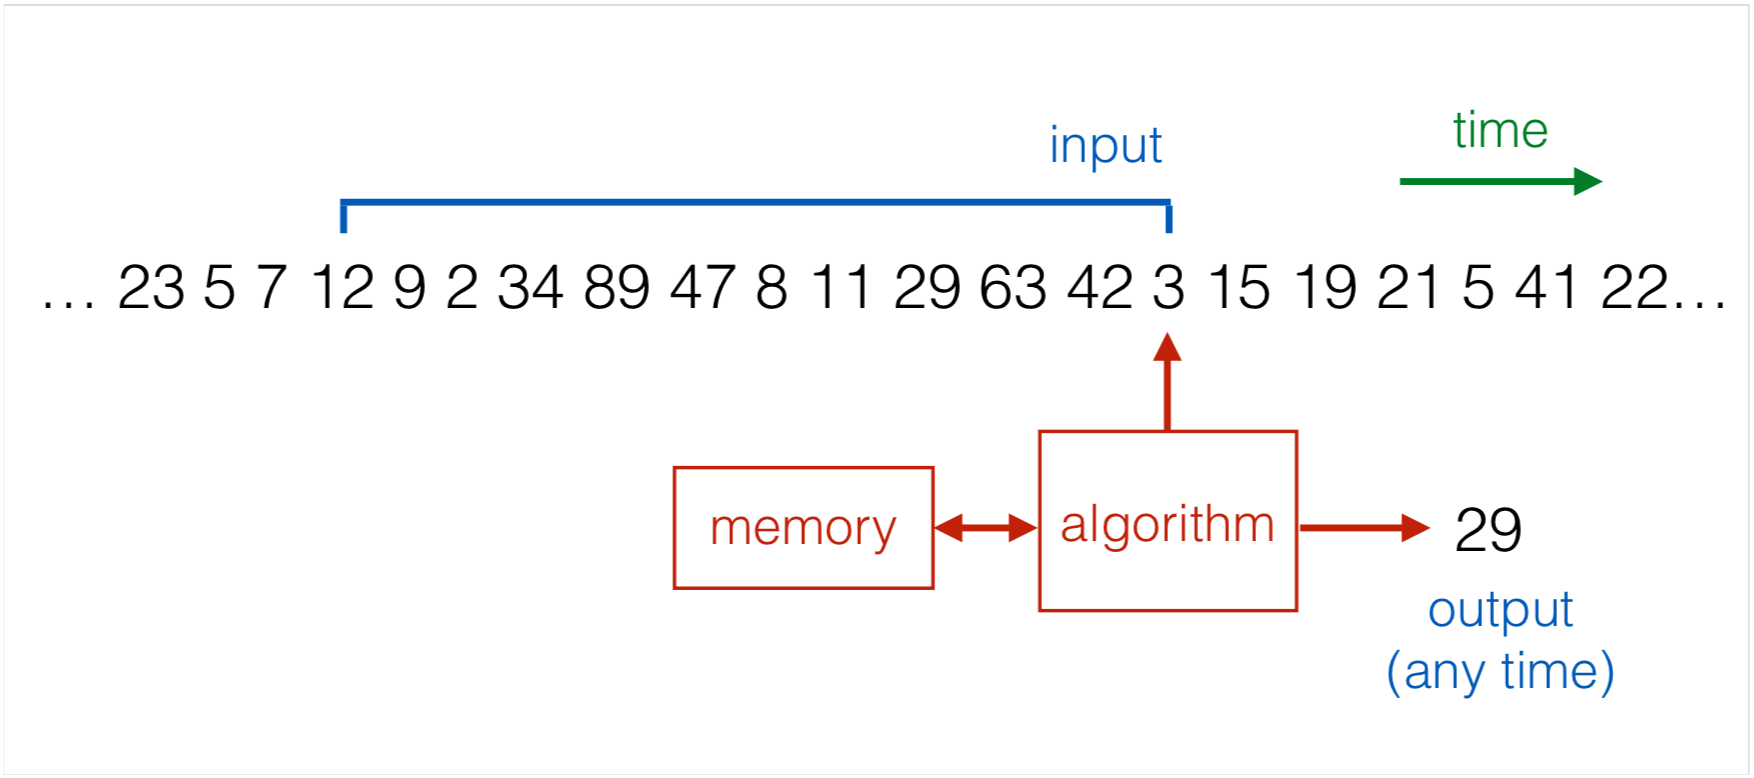
\includegraphics[width=12cm]{1_sliding_window.png}
          \captionof{figure}{Representation of sliding window: \textit{"CS-E4600 - slide set 7"}.}
        \end{center}

        Using the same logic and intuition we can argue that the \textit{priority sampling for sliding window} (shown in figure 1), will use $\mathcal{O}(\log{w}\log{n})$, where $\log{w}$ is the length of the sliding window and $\log{n}$ is the space for numbers to be stored. The arguments for our prove are the criteria that:
        \begin{itemize}
          \item in any given window each item has equal chance to be selected as a random sample
          \item each removed element has a larger element proceeding it
          \item at any given point we expect the space efficiency $\mathcal{O}(w)$ with maximal elements
          \item and finally, maintaining list of maximal elements requires  $\mathcal{O}(\log{w})$ time
        \end{itemize}
      \item \textbf{Problem:} \textit{Reservoir algorithm for sampling 1 element in a data stream:}
        \begin{enumerate}
          \item \textbf{Question}: \textit{explain k-sample in a data stream is uniform:} \\
            The meaning of $k-sample$ in a data stream being uniform is: for randomly choosing a sample of $k$ items from a data stream, at any given time each element of the data stream have equal probability of being sampled.

          \item \textbf{Question}: \textit{value of the probability p:} \\
            The value of the probability will be the length of $k-sample$ divided by the value of how many elements at current time we have seen, $t$. Which is $\dfrac{k}{t}$.

          \item \textbf{Question}: \textit{prove that value of p gives uniform samples:} \\
            Let's suppose that our $k-sample$ has 5 elements. When sixth element arrives $i=6$ and $t=[1,2...6]$, each element is kept with the probability $\dfrac{5}{6}$, which is:
            \begin{align*}
              (1)(\frac{1}{6} + (\frac{5}{6})(\frac{4}{5})) = \frac{1}{6} + \frac{4}{6} = \frac{5}{6}
            \end{align*}
            when the seventh element arrives $i=7$ and $t=[1,2...7]$, the seventh element is kept with the probability $5/7$ and each of the previous $6$ elements are also kept with the same probability. Following that logic, we can prove by induction that when there are $n$ elements, each one is kept with the probability $5/n$. Consequently, our general notation will be:
            \begin{align*}
              P(k_{sample}|t_{elements\ seen}) = \frac{k}{t}
            \end{align*}

        \end{enumerate}

      \item \textbf{Problem:} \textit{Resort to sampling of good items:}
        \begin{enumerate}
          \item \textbf{Question}: \textit{a real-world application for the algorithm:} \\
            Imagine an insurance company that operates in the US, Europe and Asia and has about 2 billion customers. By the end of every month it wants to check an estimated number of sick leaves reported by each customer for the whole period of 30 days. A traditional way would be run through all 2 billion people and check if they have reported sick leave or not for a period of 30 days. That could be computationally expensive and time consuming. Instead they could use this algorithm to take a subset of customers ($X \subseteq U$) for each day and compute how many sick leaves were reported for $i$-th day, then sum all the 30 days to get an estimated number of sick leaves reported for the past one month.\\

          \item \textbf{Question}: \textit{explain the intuition of Monte Carlo algorithm:} \\
            Referring to the example brought in $4.1$ we can explain the Monte Carlo algorithm with some assumed data. So, we have a set of 2 billion people and in the first step the Monte Carlo algorithm takes a random subset $X \subseteq U$, of size $|X|= N$:
            \begin{align*}
              U & = \{ all \ 2 \ bilion \ customers \}  \\
              X & = \{ a \ random \ subset \ of \ U \ with \ both \ good \ and \ bad \ items \} \\
              N & = length \ of \ X, \ let's \ say \ it \ is \ 20,000
            \end{align*}
            Next it takes only good items from the set $X$:
            \begin{align*}
              Y = \{ subset \ of \ X \ who \ reported \ sick \ leave, \ "good \ items" \} = \|Y\| = eg: 900
            \end{align*}

            And only after that it calculates the the estimated "good items":
            \begin{align*}
              Z = \dfrac{ |U||Y|}{N} & = \dfrac{900 * 2,000,000,000}{20000} \\
                                     & = 90,000,000 \ sick \ leaves \ reported \ per \ one \ day
            \end{align*}
            For 30 days we can do the same calculations 30 times and sum all up. \\
            As you can see the intuition is pretty straight forward once you have a real world use case for the algorithm.

          \item \textbf{Question}: \textit{explain the equation in English:} \\
            The equation:
            \begin{align*}
              Pr[(1 - \epsilon)|G| \leq Z \leq (1 + \epsilon)|G|] \geq 1 - \delta
            \end{align*}
            has several "segments" and by explaining each part we can clarify the general picture, which allows us to explicitly state what the equation stands for:

            $|G|$ - is the number good items of a universe $U$ \\
            $Z$ - estimate or approximation of $|G|$ \\
            $\epsilon$ - an error \\
            $\delta$ - a probability that $Z$ does not lie within an interval

            We then move on to the bigger parts:

            $(1 - \epsilon)|G|$ - is a lower bound for $Z$ \\
            $(1 + \epsilon)|G|$ - is an upper bound for $Z$

            Putting all these together, the equation implies that the probability that $Z$ lies between two bounds is greater than or equal to $1 - \delta$.

          \item \textbf{Question}: \textit{use the Chernoff bound to show the Monte Carlo algorithm returns an estimate Z:}
            \begin{align*}
              N \geq \dfrac{4}{e^{2} \rho}\ln \dfrac{2}{\delta}
            \end{align*}
            % As $\rho = \dfrac{|G|}{|U|}$ Let's start by replacing with
            Let's start by replacing the $Z$ with the value $\dfrac{|U||Y|}{N}$:
            \begin{align*}
              Pr[(1 - \epsilon)|G| & \leq Z \leq (1 + \epsilon)|G|] \geq 1 - \delta => \\
              Pr[(1 - \epsilon)|G| & \leq \dfrac{|U||Y|}{N} \leq (1 + \epsilon)|G|] \geq 1 - \delta
            \end{align*}
            As we know the value of $\rho$:
            \begin{align*}
              \rho = \dfrac{|G|}{|U|} \ which \ is \ |G| = \rho|U|
            \end{align*}
            Replacing the value of $|G|$ in our equation we get:
            \begin{align*}
              Pr[(1 - \epsilon)\rho|U| \leq \dfrac{|U||Y|}{N} \leq (1 + \epsilon)\rho|U|] \geq 1 - \delta
            \end{align*}
            Multiplying this equality with $\dfrac{N}{|U|}$ we get:
            \begin{align*}
              Pr[(1 - \epsilon)\rho|U| \times \dfrac{N}{|U|} \leq \dfrac{|U||Y|}{N} \times \dfrac{N}{|U|} \leq (1 + \epsilon)\rho|U| \times \dfrac{N}{|U|}] \geq 1 - \delta
            \end{align*}
            We get:
            \begin{align*}
              Pr[(1 - \epsilon)\rho N \leq |Y| \leq (1 + \epsilon)\rho N] \geq 1 - \delta \numberthis \label{eqn}
            \end{align*}
            Before moving forward it is good time to state the Chernoff bound general notation:
            \begin{align*}
              Pr[X \geq (1 + \delta) \mu] \leq e^{ -\frac{ \delta^2 \mu }{3} } \\
              Pr[X \leq (1 - \delta) \mu] \leq e^{ -\frac{ \delta^2 \mu }{2} }
            \end{align*}
            Let's now assume that $X=Y$, $\mu = \rho N$ and $1-\delta$:
            \begin{align*}
              Pr[Y \geq (1 + \epsilon) \rho N] \leq e^{ -\frac{ \epsilon^2 \rho N }{3} } \\
              Pr[Y \leq (1 - \epsilon) \rho N] \leq e^{ -\frac{ \epsilon^2 \rho N }{2} }
            \end{align*}
            Now, let's come back to the equation $(1)$ and combine it with the Chernoff bound:
            \begin{align*}
              Pr[(1 - \epsilon)\rho N \leq |Y| \leq (1 + \epsilon)\rho N] \geq 1 - e^{ -\frac{ \epsilon^2 \rho N }{3}} - e^{ -\frac{ \epsilon^2 \rho N }{2}} \numberthis \label{eqn}
            \end{align*}
            Since
            \begin{align*}
              e^{ -\frac{ \epsilon^2 \rho N }{3}} < e^{ -\frac{ \epsilon^2 \rho N }{4}} \\
              and \\
              e^{ -\frac{ \epsilon^2 \rho N }{2}} < e^{ -\frac{ \epsilon^2 \rho N }{4}}
            \end{align*}
            We can rewrite the equation in (2) like:
            \begin{align*}
              1 - e^{ -\frac{ \epsilon^2 \rho N }{4}} - e^{ -\frac{ \epsilon^2 \rho N }{4}} & \leq 1 - \delta \leq 1 \\
              2e^{ -\frac{ \epsilon^2 \rho N }{4}} & \leq \delta \\
              \dfrac{2}{\delta}  & \leq e^{ -\frac{ \epsilon^2 \rho N }{4}} \\
              taking \ ln \ from \ both \ sides \ results \ in: \\
              ln\dfrac{2}{\delta}  & \leq \frac{ \epsilon^2 \rho N }{4} \\
              which \ is \ equivalent \ to:\
              N & \geq \dfrac{4}{\epsilon^2 \rho}ln\dfrac{2}{\delta}
            \end{align*}

          \item \textbf{Question}: \textit{discuss the bound:} \\
            If we increase the value of $N$ then the error rate decreases. If $\epsilon$ and $\delta$ are constant and $\rho$ is \textbf{small} then $N$ size should be big. On the other hand if $\epsilon$ and $\delta$ are constant and $\rho$ is \textbf{big} then $N$ size should be small.
            If $\rho$ is constant then we have these conditions:

            1. When $\epsilon$ is constant and $\delta$ changes:\\
            \begin{tabular}{c | c | c}
              $\epsilon$ & $\delta$ & $\dfrac{4}{\epsilon^2 \rho}ln\dfrac{2}{\delta}$ \\ \hline
              0.2  &  0.1     &   2995.73 \\
              0.2  &  0.05    &   3688.87 \\
              0.2  &  0.01    &   5298.31 \\
              0.2  &  0.001   &   7600.90 \\
            \end{tabular}

            2. When $\delta$ is constant and $\epsilon$ changes:\\
            \begin{tabular}{c | c | c}
              $\epsilon$ & $\delta$ & $\dfrac{4}{\epsilon^2 \rho}ln\dfrac{2}{\delta}$ \\ \hline
              0.2  &   0.1    &   2995.7 \\
              0.3  &   0.1    &   1331.4 \\
              0.4  &   0.1    &   748.9 \\
              0.5  &   0.1    &   479.3 \\
            \end{tabular}
        \end{enumerate}
    \end{enumerate}
\end{document}

